\documentclass[11pt]{article}
\usepackage{acl2012}
\usepackage{times}
\usepackage{latexsym}
\usepackage{amsmath}
\usepackage{multirow}
\usepackage{url}
\usepackage{graphicx}
\usepackage[usenames,dvipsnames]{pstricks}
\usepackage{epsfig}
\DeclareMathOperator*{\argmax}{arg\,max}
\setlength\titlebox{6.5cm}    % Expanding the titlebox

\newcommand{\spectralResult}{59.41}
\newcommand{\collapseResult}{70.82}

\title{A Paradigmatic Model for Learning Syntactic Categories}

\author{First Author \\
  Affiliation / Address line 1 \\
  Affiliation / Address line 2 \\
  Affiliation / Address line 3 \\
  {\tt email@domain} \\\And
  Second Author \\
  Affiliation / Address line 1 \\
  Affiliation / Address line 2 \\
  Affiliation / Address line 3 \\
  {\tt email@domain} \\\And
  Third Author \\
  Affiliation / Address line 1 \\
  Affiliation / Address line 2 \\
  Affiliation / Address line 3 \\
  {\tt email@domain} \\}

\date{}

\begin{document}
\maketitle
\begin{abstract}

We investigate paradigmatic representations of word context in the
domain of unsupervised syntactic category acquisition.  Paradigmatic
representations of word context are based on potential substitutes of
a word in contrast to syntagmatic representations based on properties
of neighboring words.  We compare a bigram based baseline model with
several paradigmatic models and demonstrate significant gains in
accuracy.  Our best model based on Euclidean co-occurrence embedding
combines the paradigmatic context representation with morphological
and orthographic features and achieves 80\% many-to-one accuracy on a
45-tag 1M word corpus.
\end{abstract}

\section{Introduction}
\label{sec:intro}

Grammar rules apply not to individual words (e.g. dog, eat) but to
syntactic categories of words (e.g. noun, verb).  Thus constructing
syntactic categories (also known as lexical or part-of-speech
categories) is one of the fundamental problems in language
acquisition.

Syntactic categories represent groups of words that can be substituted
for one another without altering the grammaticality of a sentence.
Linguists identify syntactic categories based on semantic, syntactic,
and morphological properties of words.  There is also evidence that
children use prosodic and phonological features to bootstrap syntactic
category acquisition \cite{ambridge2011child}.  However there is as
yet no satisfactory computational model that can match human
performance.  Thus identifying the best set of features and best
learning algorithms for syntactic category acquisition is still an
open problem.

\begin{figure}[b] \centering
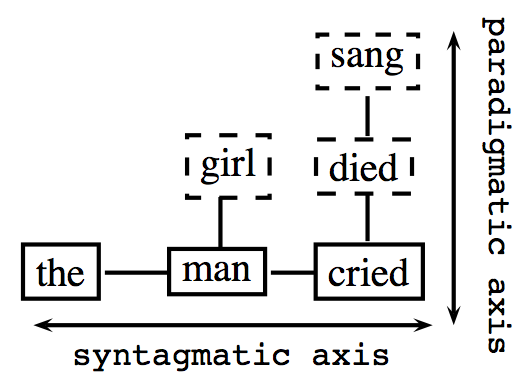
\includegraphics[width=50mm]{paradigmatic.png}
% % Generated with LaTeXDraw 2.0.8
% Tue Jan 10 15:57:06 EET 2012
% \usepackage[usenames,dvipsnames]{pstricks}
% \usepackage{epsfig}
% \usepackage{pst-grad} % For gradients
% \usepackage{pst-plot} % For axes
\scalebox{1} % Change this value to rescale the drawing.
{
\begin{pspicture}(0,-1.6728125)(4.73474,1.6528125)
\usefont{T1}{ptm}{m}{n}
\rput(0.39520833,-0.6571875){\psframebox[linewidth=0.04]{the}}
\usefont{T1}{ptm}{m}{n}
\rput(1.8816146,-0.6571875){\psframebox[linewidth=0.04]{man}}
\usefont{T1}{ptm}{m}{n}
\rput(1.9886458,0.3428125){\psframebox[linewidth=0.04,linestyle=dashed,dash=0.16cm 0.16cm]{girl}}
\usefont{T1}{ptm}{m}{n}
\rput(3.3298957,-0.6571875){\psframebox[linewidth=0.04]{cried}}
\usefont{T1}{ptm}{m}{n}
\rput(3.2798958,0.3428125){\psframebox[linewidth=0.04,linestyle=dashed,dash=0.16cm 0.16cm]{died}}
\usefont{T1}{ptm}{m}{n}
\rput(3.3158333,1.3428125){\psframebox[linewidth=0.04,linestyle=dashed,dash=0.16cm 0.16cm]{sang}}
\usefont{T1}{pcr}{m}{n}
\rput(2.020677,-1.4671875){\footnotesize syntagmatic axis}
\usefont{T1}{pcr}{m}{n}
\rput{-90.0}(4.4150524,4.661927){\rput(4.507552,0.1328125){\footnotesize paradigmatic axis}}
\psline[linewidth=0.04cm,arrowsize=0.05291667cm 2.0,arrowlength=1.4,arrowinset=0.4]{<->}(0.13364583,-1.1671875)(3.9336457,-1.1671875)
\psline[linewidth=0.04cm,arrowsize=0.05291667cm 2.0,arrowlength=1.4,arrowinset=0.4]{<->}(4.133646,1.6328125)(4.133646,-1.1671875)
\psline[linewidth=0.04cm](0.81364584,-0.6671875)(1.4136459,-0.6671875)
\psline[linewidth=0.04cm](2.3936458,-0.6671875)(2.8136458,-0.6671875)
\psline[linewidth=0.04cm](1.9136459,0.0528125)(1.9136459,-0.4271875)
\psline[linewidth=0.04cm](3.3136458,0.0928125)(3.3136458,-0.3671875)
\psline[linewidth=0.04cm](3.3136458,1.0128125)(3.3136458,0.6328125)
\end{pspicture} 
}

\caption{Syntagmatic vs. paradigmatic axes for words in a simple
  sentence \cite{chandler2007semiotics}.}
\label{fig:paradigmatic}
\end{figure}

Relationships between linguistic units can be classified into two
types: syntagmatic (concerning positioning), and paradigmatic
(concerning substitution).  Syntagmatic relations determine which
units can combine to create larger groups and paradigmatic relations
determine which units can be substituted for one another.
Figure~\ref{fig:paradigmatic} illustrates the paradigmatic vs
syntagmatic axes for words in a simple sentence and their possible
substitutes.  

In this study, we represent the paradigmatic axis directly by building
{\em substitute vectors} for each word position in the text.  The
dimensions of a substitute vector represent words in the vocabulary,
and the magnitudes represent the probability of occurrence in the given
position.  Note that the substitute vector for a word position (e.g.
the second word in Fig.~\ref{fig:paradigmatic}) is a function of the
context only (i.e. ``the \_\_\_ cried''), and does not depend on the
word that does actually appear there (i.e. ``man'').  Thus substitute
vectors represent {\em individual word contexts}, not word types.  We
refer to the use of features based on substitute vectors as 
{\em paradigmatic representations of word context}.

Our preliminary experiments indicated that using context information
alone without the identity or the features of the target word
(e.g. using dimensionality reduction and clustering on substitute
vectors) has limited success and modeling the co-occurrence of word
and context types is essential for inducing syntactic categories.  In
the models presented in this paper, we combine paradigmatic
representations of word context with features of co-occurring words
within the co-occurrence data embedding (CODE) framework
\cite{globerson2007euclidean,maron2010sphere}.  The resulting
embeddings for word types are split into 45 clusters using k-means and
the clusters are compared to the 45 gold tags in the 1M word Penn
Treebank Wall Street Journal corpus \cite{treebank3}.  We obtain
many-to-one accuracies up to .7680 using only distributional
information (the identity of the word and a representation of its
context) and .8023 using morphological and orthographic features of
words improving the state-of-the-art in unsupervised part-of-speech
tagging performance.

% example substitute vectors (both syntactic and semantic)
The high probability substitutes reflect both semantic and syntactic
properties of the context as seen in the example below (the numbers in
parentheses give substitute probabilities):

\begin{quotation}
\noindent {\em ``Pierre Vinken, 61 years old, will join the board as a nonexecutive director Nov.~29.''}\\

\noindent {\bf the:} its (.9011), the (.0981), a (.0006), $\ldots$\\
{\bf board:} board (.4288), company (.2584), firm (.2024), bank (.0731), $\ldots$
\end{quotation}

Top substitutes for the word ``the'' consist of words that can act as
determiners.  Top substitutes for ``board'' are not only nouns, but
specifically nouns compatible with the semantic context.

This example illustrates two concerns inherent in all distributional
methods: (i) words that are generally substitutable like ``the'' and
``its'' are placed in separate categories ({\sc dt} and {\sc prp\$})
by the gold standard, (ii) words that are generally not substitutable
like ``do'' and ``put'' are placed in the same category ({\sc vb}).
Freudenthal et al. \shortcite{freudenthal2005resolution} point out
that categories with unsubstitutable words fail the standard
linguistic definition of a syntactic category and children do not seem
to make errors of substituting such words in utterances
(e.g. {\em``What do you want?''}  vs. {\em *``What put you want?''}).
Whether gold standard part-of-speech tags or distributional categories
are better suited to applications like parsing or machine translation
can be best decided using extrinsic evaluation.  However in this study
we follow previous work and evaluate our results by comparing them to
gold standard part-of-speech tags.

Section~\ref{sec:related} gives a detailed review of related work.
Section~\ref{sec:lm} describes the dataset and the construction of the
substitute vectors.  Section~\ref{sec:code} describes co-occurrence
data embedding, the learning algorithm used in our experiments.
Section~\ref{sec:exp} describes our experiments and compares our
results with previous work.  Section~\ref{sec:discuss} gives a brief
error analysis and Section~\ref{sec:contrib} summarizes our
contributions.  All the data and the code to replicate the results
given in this paper is available from the authors' website at
\mbox{\url{http://goo.gl/RoqEh}}.


%% Computational models of syntactic category acquisition rely mainly on
%% distributional analysis: Words that share the same distribution
%% (i.e. that occur in the same context) are grouped into the same
%% category.  The definition of ``the same context'' vary across studies.
%% Algorithms based on the Hidden Markov Model use class based n-grams to
%% specify context \cite{Brown:1992:CNG:176313.176316}, others use a
%% frame of neighboring words around the target word
%% \cite{Schutze:1995:DPT:976973.976994}.

%% Our hypothesis is that potential substitutes of a word are directly
%% indicative of its syntactic category and should be useful in acquiring
%% syntactic categories in general.  

%% Our main contribution in this study
%% is to introduce paradigmatic features, i.e. features based on
%% potential substitutes of the target word, to represent word context.

%% Both syntagmatic and paradigmatic relations of a word can be used to
%% represent its context.  In the syntagmatic case the context is
%% represented by a selection of neighboring words, in the paradigmatic
%% case it is represented by a set of possible substitutes.  In previous
%% studies of syntactic category learning the context representation has
%% been primarily syntagmatic, either implicit in the class based n-grams
%% of the standard Hidden Markov Model, or explicit in the construction
%% and clustering of left and right neighbors.

%% In this study we explore a paradigmatic representation of the context
%% of a word in syntactic category acquisition.  Specifically, the
%% context of a word is represented by a list of its possible substitutes
%% and their probabilities, which we call the {\em substitute vector}.
%% Note that the substitute vector is a function of the context only, not
%% the target word.  Thus in effect we are clustering contexts, not
%% words.  When word contexts are clustered based on their substitute
%% vectors they reveal a grouping that largely match the traditional part
%% of speech boundaries (\bestResult many-to-one score using a
%% 45-tag 24K word test corpus).
%% % standard HMM-EM gives 42\% on the same data.

%% Section~\ref{sec:related} gives a detailed review of related work.
%% The construction of the substitute vectors is described in
%% Section~\ref{sec:lm}.  To find out how to best make use of this new
%% paradigmatic representation, we explore different distance metrics
%% (Section~\ref{sec:dist}), dimensionality reduction methods
%% (Section~\ref{sec:dimreduce}), and clustering algorithms
%% (Section~\ref{sec:clustering}) for substitute vectors.  We note that
%% close to 95\% of the word occurrences in human labeled data are tagged
%% with their most frequent part of speech
%% \cite{Lee:2010:STU:1870658.1870741}, making one-tag-per-word a fairly
%% good first approximation.  Even ambicategory words generally have
%% fairly skewed part of speech distributions.
%% Section~\ref{sec:sparsity} looks at ways to increase the sparsity of
%% our solutions and demonstrates significant improvements using the
%% one-tag-per-word assumption and similarity metrics that introduce
%% sparsity.  Section~\ref{sec:discussion} discusses the results and
%% Section~\ref{sec:contrib} summarizes our contributions.



\section{Related Work}
\label{sec:related}
%%% This part looks fine
There are several good reviews of algorithms for unsupervised
part-of-speech induction
\cite{Christodoulopoulos:2010:TDU:1870658.1870714,Gao:2008:CBE:1613715.1613761}
and models of syntactic category acquisition \cite{ambridge2011child}.

This work is to be distinguished from supervised part-of-speech
disambiguation systems, which use labeled training data
\cite{Church:1988:SPP:974235.974260}, unsupervised disambiguation
systems, which use a dictionary of possible tags for each word
\cite{Merialdo:1994:TET:972525.972526}, or prototype driven systems
which use a small set of prototypes for each class
\cite{Haghighi:2006:PLS:1220835.1220876}.  The problem of induction is
important for studying under-resourced languages that lack labeled
corpora and high quality dictionaries.  It is also essential in
modeling child language acquisition because every child manages to
induce syntactic categories without access to labeled sentences,
labeled prototypes, or dictionary constraints.
%%%%
%\paragraph{Distributional vs. Feature Based}
% \subsection{Distributional vs. Feature Based}

Models of unsupervised part-of-speech induction fall into two broad
groups based on the information they utilize.  Distributional models
only use word types and their context statistics.  Word-feature models
incorporate additional morphological and orthographic features.

\subsection{Distributional models}

Distributional models can be further categorized into three subgroups
based on the learning algorithm.  The first subgroup represents each
word type with its context vector and clusters these vectors
accordingly \cite{Schutze:1995:DPT:976973.976994}.  Work in modeling
child syntactic category acquisition has generally followed this
clustering approach
\cite{redington1998distributional,mintz2003frequent}.  The second
subgroup consists of probabilistic models based on the Hidden Markov
Model (HMM) framework \cite{Brown:1992:CNG:176313.176316}.  A third
group of algorithms constructs a low dimensional representation of the
data that represents the empirical co-occurrence statistics of word
types \cite{globerson2007euclidean}, which is covered in more detail
in Section~\ref{sec:code}.

\paragraph{Clustering:}
Clustering based methods represent context using neighboring words,
typically a single word on the left and a single word on the right
called a ``frame'' (e.g., {\em {\bf the} dog {\bf is}; {\bf the} cat
  {\bf is}}).  They cluster word types rather than word tokens based
on the frames they occupy thus employing one-tag-per-word assumption
from the beginning (with the exception of some methods in
\cite{Schutze:1995:DPT:976973.976994}).  They may suffer from data
sparsity caused by infrequent words and infrequent contexts.  The
solutions suggested either restrict the set of words and set of
contexts to be clustered to the most frequently observed, or use
dimensionality reduction.  Redington et
al. \shortcite{redington1998distributional} define context similarity
based on the number of common frames bypassing the data sparsity
problem but achieve mediocre results.  Mintz
\shortcite{mintz2003frequent} only uses the most frequent 45 frames
and Biemann \shortcite{biemann2006unsupervised} clusters the most
frequent 10,000 words using contexts formed from the most frequent
150-200 words.  Sch\"utze \shortcite{Schutze:1995:DPT:976973.976994}
and Lamar et al. \shortcite{lamar-EtAl:2010:Short} employ SVD to enhance
similarity between less frequently observed words and contexts.  Lamar
et al. \shortcite{Lamar:2010:LCU:1870658.1870736} represent each
context by the currently assigned left and right tag (which eliminates
data sparsity) and cluster word types using a soft k-means style
iterative algorithm.  They report the best clustering result to date
of .708 many-to-one accuracy on a 45-tag 1M word corpus.
% all except schutze cluster word types

\paragraph{HMMs:}
The prototypical bitag HMM model maximizes the likelihood of the
corpus $w_1 \ldots w_n$ expressed as $P(w_1|c_1)\prod_{i=2}^n
P(w_i|c_i) P(c_i|c_{i-1})$ where $w_i$ are the word tokens and $c_i$
are their (hidden) tags.  One problem with such a model is its
tendency to distribute probabilities equally and the resulting
inability to model highly skewed word-tag distributions observed in
hand-labeled data \cite{johnson:2007:EMNLP-CoNLL2007}.  To favor
sparse word-tag distributions one can enforce a strict
one-tag-per-word solution
\cite{Brown:1992:CNG:176313.176316,Clark:2003:CDM:1067807.1067817},
use sparse priors in a Bayesian setting
\cite{goldwater-griffiths:2007:ACLMain,johnson:2007:EMNLP-CoNLL2007},
or use posterior regularization
\cite{Ganchev:2010:PRS:1859890.1859918}.  Each of these techniques
provide significant improvements over the standard HMM model: for
example Gao and Johnson \shortcite{Gao:2008:CBE:1613715.1613761} show
that sparse priors can gain from 4\% (.62 to .66 with a 1M word
corpus) in cross-validated many-to-one accuracy.  However
Christodoulopoulos et
al. \shortcite{Christodoulopoulos:2010:TDU:1870658.1870714} show that
the older one-tag-per-word models such as
\cite{Brown:1992:CNG:176313.176316} outperform the more sophisticated
sparse prior and posterior regularization methods both in speed and
accuracy (the Brown model gets .68 many-to-one accuracy with a 1M word
corpus).  Given that close to 95\% of the word occurrences in human
labeled data are tagged with their most frequent part of speech
\cite{Lee:2010:STU:1870658.1870741}, this is probably not surprising;
one-tag-per-word is a fairly good first approximation for induction.

%% \paragraph{Co-occurrence embedding:}
%% Embedding algorithms maps the original data to a lower dimensional
%% space that preserves certain similarity structure defined between the
%% objects in the data.  However in real life problems such as POS
%% induction the similarity between contexts and word types can not be
%% trivially constructed given that only the co-occurrence information
%% exists between word types and their contexts.
%% S-Code\cite{NIPS2010_1196} which is a spherical extension of
%% \cite{Globerson:2007:EEC:1314498.1314572} algorithm maps the
%% word-types and their contexts on to a low dimensional Euclidean sphere
%% while preserving the co-occurrence statistics between them and then
%% clusters the low dimensional data with k-means algorithm.  They report
%% .688 many-to-one accuracy on a 45-tag 1M word corpus.

\subsection{Word-feature models}
One problem with the algorithms in the previous section is the poverty
of their input features.  Of the syntactic, semantic, and
morphological information linguists claim underlie syntactic
categories, context vectors or bitag HMMs only represent limited
syntactic information in their input.  Experiments incorporating
morphological and orthographic features into HMM based models
demonstrate significant improvements.
\cite{Clark:2003:CDM:1067807.1067817,bergkirkpatrick-klein:2010:ACL,blunsom-cohn:2011:ACL-HLT2011}
incorporate similar orthographic features and report improvements of
3, 7, and 10\% respectively over the baseline Brown model.
Christodoulopoulos et
al. \shortcite{Christodoulopoulos:2010:TDU:1870658.1870714} use
prototype based features as described in
\cite{Haghighi:2006:PLS:1220835.1220876} with automatically induced
prototypes and report an 8\% improvement over the baseline Brown
model.  Christodoulopoulos et
al. \shortcite{christodoulopoulos-goldwater-steedman:2011:EMNLP}
define a type-based Bayesian multinomial mixture model in which each
word instance is generated from the corresponding word type mixture
component and word contexts are represented as features.  They achieve
a .728 \mto score by extending their model with additional
morphological and alignment features gathered from parallel corpora.
To our knowledge, nobody has yet tried to incorporate phonological or
prosodic features in a computational model for syntactic category
acquisition.

\subsection{Paradigmatic representations}

Sahlgren \shortcite{sahlgren2006word} gives a detailed analysis of
paradigmatic and syntagmatic relations in the context of word-space
models used to represent word meaning.  Sahlgren's paradigmatic model
represents word types using co-occurrence counts of their frequent
neighbors, in contrast to his syntagmatic model that represents word
types using counts of contexts (documents, sentences) they occur in.
Our substitute vectors do not represent word types at all, but {\em
  contexts of word tokens} using probabilities of likely substitutes.
Sahlgren finds that in word-spaces built by frequent neighbor vectors,
more nearest neighbors share the same part-of-speech compared to
word-spaces built by context vectors.  We find that representing the
paradigmatic axis more directly using substitute vectors rather than
frequent neighbors improve part-of-speech induction.

Our paradigmatic representation is also related to the second order
co-occurrences used in \cite{Schutze:1995:DPT:976973.976994}.
Sch{\"u}tze concatenates the left and right context vectors for the
target word type with the left context vector of the right neighbor
and the right context vector of the left neighbor.  The vectors from
the neighbors include potential substitutes.  Our method improves on
his foundation by using a 4-gram language model rather than bigram
statistics, using the whole 78,498 word vocabulary rather than the
most frequent 250 words.  More importantly, rather than simply
concatenating vectors that represent the target word with vectors that
represent the context we use S-CODE to model their co-occurrence
statistics.

\subsection{Evaluation}
%% It is natural to question the merit of evaluating unsupervised results
%% by comparing them to gold standard tags.  For example
%% \cite{freudenthal2005resolution} argue that a verb category (such as
%% {\sc vb} in Penn Treebank) that contains verbs that can and cannot be
%% used in certain constructions (e.g. the imperative) and verbs that can
%% be used as both auxiliaries and main verbs (e.g., {\em do, have}) does
%% not in fact constitute a set of items that could be substituted for
%% one another in particular sentences.  Such a category fails the
%% standard linguistic definition of a syntactic category and children do
%% not seem to make errors of substituting such words in utterances
%% (e.g. {\em''What do you want?''} vs. {\em *''What put you want?''}).
%% They suggest evaluating models by incorporating a production component
%% that allows the model's output to be compared to speech produced by
%% children exposed to the same input.  \cite{frank2009evaluating},
%% motivated by the lack of gold standards for many novel languages,
%% suggest comparing a system's clusters to a set of clusters created
%% from {\em substitutable frames}.  They create frames using two words
%% appearing in the corpus with exactly one word between and calculate
%% precision, recall, and F-score of the system's clustering.
%% Statistical parsers or factored machine learning systems could also be
%% sources of extrinsic evaluation for induced syntactic categories.  We
%% hope such extrinsic evaluation will be more widespread in the future
%% but nevertheless use many-to-one (\mto) and V-measure (\vm) metric on
%% the 45-tag Penn Treebank gold standard to evaluate the current work.

We report many-to-one and V-measure scores for our experiments as
suggested in \cite{Christodoulopoulos:2010:TDU:1870658.1870714}.  The
many-to-one (MTO) evaluation maps each cluster to its most frequent
gold tag and reports the percentage of correctly tagged instances.
The \mto score naturally gets higher with increasing number of
clusters but it is an intuitive metric when comparing results with the
same number of clusters.  The V-measure (VM) \cite{rosenberg2007v} is
an information theoretic metric that reports the harmonic mean of
homogeneity (each cluster should contain only instances of a single
class) and completeness (all instances of a class should be members of
the same cluster).  In Section~\ref{sec:discuss} we argue that
homogeneity is perhaps more important in part-of-speech induction and
suggest \mto with a fixed number of clusters as a more intuitive
metric.

%% \paragraph{Many-to-one (MTO)} metric measures the cluster purity 
%% therefore each cluster is mapped to the most frequent gold tag of the
%% words observed in that cluster.  \mto metric is the most intuitive
%% measure, however it has a bias towards to the increasing number of
%% clusters thus it should be used when the number of clusters is fixed
%% \cite{christodoulopoulos-goldwater-steedman:2011:EMNLP}.
%% \paragraph{V-measure (VM)} is an entropy based metric that calculates
%% weighted average of cluster homogeneity and completeness in a similar
%% fashion with F-measure recall and precision, respectively.  The
%% cluster homogeneity is an analogy of the cluster purity in \mto.
%% Although \vm is more robust to variable number of clusters, it is less
%% intuitive than \mto
%% \cite{christodoulopoulos-goldwater-steedman:2011:EMNLP}.  Moreover it
%% punishes the clustering when words with same gold tag distributed over
%% different clusters which contradicts with the idea of POS induction
%% since the aim is to cluster words according to the underlying natural
%% grouping.

%%% DY: where is the original paper that introduced V-measure?
%%% DY: are you sure Chris2011 is the right citation, shouldn't it be Chris2010?


\section{Substitute Vectors}
\label{sec:lm}

In this study, we predict the part of speech of a word in a given
context based on its substitute vector.  The dimensions of the
substitute vector represent words in the vocabulary, and the entries
in the substitute vector represent the probability of those words
being used in the given context.  Note that the substitute vector is a
function of the context only and is indifferent to the target word.
This section details the choice of the data set, the vocabulary and
the estimation of substitute vector probabilities.

% what is the test data
The Wall Street Journal Section of the Penn Treebank \cite{treebank3}
was used as the test corpus (1,173,766 tokens, 49,206 types).
% what is the tag set
The treebank uses 45 part-of-speech tags which is the set we used as
the gold standard for comparison in our experiments.
% what is the LM training data
%Train => 5181717 126019973 690121813
To compute substitute probabilities we trained a language model using
approximately 126 million tokens of Wall Street Journal data
(1987-1994) extracted from CSR-III Text \cite{csr3text} (we excluded
the test corpus).
% how is the language model trained
We used SRILM \cite{Stolcke2002} to build a 4-gram language model with
Kneser-Ney discounting.
% what is the vocabulary
Words that were observed less than 20 times in the language model training data
were replaced by \textsc{unk} tags, which gave us a vocabulary size of
78,498.
% perplexity
The perplexity of the 4-gram language model on the test corpus is 96.

% how are the substitutes computed
It is best to use both left and right context when estimating the
probabilities for potential lexical substitutes.  For example, in
\emph{``He lived in San Francisco suburbs.''}, the token \emph{San}
would be difficult to guess from the left context but it is almost
certain looking at the right context.  We define $c_w$ as the $2n-1$
word window centered around the target word position: $w_{-n+1} \ldots
w_0 \ldots w_{n-1}$ ($n=4$ is the n-gram order).  The probability of a
substitute word $w$ in a given context $c_w$ can be estimated as:
\begin{eqnarray}
  \label{eq:lm1}P(w_0 = w | c_w) & \propto & P(w_{-n+1}\ldots w_0\ldots w_{n-1})\\
  \label{eq:lm2}& = & P(w_{-n+1})P(w_{-n+2}|w_{-n+1})\nonumber\\
  &&\ldots P(w_{n-1}|w_{-n+1}^{n-2})\\
  \label{eq:lm3}& \approx & P(w_0| w_{-n+1}^{-1})P(w_{1}|w_{-n+2}^0)\nonumber\\
  &&\ldots P(w_{n-1}|w_0^{n-2})
\end{eqnarray}
where $w_i^j$ represents the sequence of words $w_i w_{i+1} \ldots
w_{j}$.  In Equation \ref{eq:lm1}, $P(w|c_w)$ is proportional to
$P(w_{-n+1}\ldots w_0 \ldots w_{n+1})$ because the words of the
context are fixed.  Terms without $w_0$ are identical for each
substitute in Equation \ref{eq:lm2} therefore they have been dropped
in Equation \ref{eq:lm3}.  Finally, because of the Markov property of
n-gram language model, only the closest $n-1$ words are used in the
experiments.

Near the sentence boundaries the appropriate terms were truncated in
Equation \ref{eq:lm3}.  Specifically, at the beginning of the sentence
shorter n-gram contexts were used and at the end of the sentence terms
beyond the end-of-sentence token were dropped.

For computational efficiency only the top 100 substitutes and their
unnormalized probabilities were computed for each of the 1,173,766
positions in the test set\footnote{The substitutes with unnormalized
  log probabilities can be downloaded from \mbox{\url{http://goo.gl/jzKH0}}.
  For a description of the {\sc fastsubs} algorithm used to generate
  the substitutes please see \mbox{\url{http://arxiv.org/abs/1205.5407v1}}.
  {\sc fastsubs} accomplishes this task in about 5 hours, a naive
  algorithm that looks at the whole vocabulary would take more than 6
  days on a typical 2012 workstation.}.  The probability vectors for
each position were normalized to add up to 1.0 giving us the final
substitute vectors used in the rest of this study.



%%

%%

%%

%%

\section{Error Analysis}
\label{sec:discuss}

Figure~\ref{plot-hinton} is the Hinton diagram showing the
relationship between the most frequent tags and clusters from the
experiment in Section~\ref{sec:feat}.  In general the errors seem to
be the lack of completeness (multiple large entries in a row), rather
than lack of homogeneity (multiple large entries in a column).  The
algorithm tends to split large word classes into several clusters.
Some examples are:
\begin{itemize}
\item Titles like Mr., Mrs., and Dr. are split from the rest of the
  proper nouns in cluster (39).
\item Auxiliary verbs (10) and the verb ``say'' (22) have been split
  from the general verb clusters (12) and (7).
\item Determiners ``the'' (40), ``a'' (15), and capitalized
  ``The'', ``A'' (6) have been split into their own clusters.
\item Prepositions ``of'' (19), and ``by'', ``at'' (17) have been
  split from the general preposition cluster (8).
\end{itemize}
Nevertheless there are some homogeneity errors as well:
\begin{itemize} 
\item The adjective cluster (5) also has some noun members probably
  due to the difficulty of separating noun-noun compounds from
  adjective modification.
\item Cluster (6) contains capitalized words that span a number of
  categories.
\end{itemize}

Most closed-class items are cleanly separated into their own clusters
as seen in the lower right hand corner of the diagram.  The
completeness errors are not surprising given that the words that have
been split are not generally substitutable with the other members of
their Penn Treebank category.  Thus it can be argued that metrics that
emphasize homogeneity such as \mto are more appropriate in this
context than metrics that average homogeneity and completeness such as
\vm as long as the number of clusters is controlled.


\section{Contributions}
\label{sec:contrib}

We introduced a paradigmatic representation for word context which
contains possible substitutes for the target word and their
probabilities.  The substitute probabilities were estimated using a
standard 4-gram language model with Kneser-Ney smoothing.  We
investigated distance metrics, dimensionality reduction techniques and
clustering algorithms appropriate for substitute probability vectors
and evaluated them using a supervised k-nearest-neighbor baseline and
many-to-one accuracy relative to a 45-tag 24K word test corpus.  We
found that the KL2 distance metric (a symmetric version of
Kullback-Leibler divergence), dimensionality reduction using Laplacian
eigenmaps, and spectral clustering work well with substitute vectors.
Spectral clustering of substitute vectors reveal a grouping that
largely match traditional part of speech boundaries (\spectralResult\%
many-to-one accuracy) which further improve when the one-tag-per-word
constraint is imposed (\collapseResult\% many-to-one accuracy).  These
results compare favorably to previous results published for the 45-tag
24K word test corpus we have used.  
%% We are investigating ways to speed up the algorithm so it can be tested on larger corpora.


\bibliographystyle{acl2012}
\bibliography{posind2012}
\end{document}
